%----------------------------------------------------------------------------------------
%    PACKAGES AND THEMES
%----------------------------------------------------------------------------------------

\documentclass[aspectratio=169,xcolor=dvipsnames]{beamer}
\usetheme{SimpleDarkBlue}

\usepackage{hyperref}
\usepackage{graphicx} % Allows including images
\graphicspath{{./images/}}
\usepackage{booktabs} % Allows the use of \toprule, \midrule and \bottomrule in tables
\usepackage{csquotes}
\usepackage{animate}

%----------------------------------------------------------------------------------------
%    TITLE PAGE
%----------------------------------------------------------------------------------------

\title{Convex Optimization Relaxation for Radial Image Reconstruction}
% \subtitle{Subtitle}

\author{
    Mincu Adrian-Lucian\\
    \small Coordonator științific: Conf. Dr. Rusu Cristian
}

\institute
{
    Universitatea din București - Facultatea de Matematică și Informatică
}
\date{Iulie, 2025} % Date, can be changed to a custom date

%----------------------------------------------------------------------------------------
%    PRESENTATION SLIDES
%----------------------------------------------------------------------------------------

\begin{document}

\begin{frame}
    % Print the title page as the first slide
    \titlepage
\end{frame}

%------------------------------------------------
\section{Introducere}

\begin{frame}{Introducere}
    \begin{columns}
        \begin{column}{0.6\textwidth}
            \textbf{Motivație}
            \begin{itemize}
                \item CT: \textbf{375+ mil. scanări/an}, bazate pe Radon, cu +\textbf{3–4\%} anual.
                \item Transformata Radon este studiată atât în matematică, cât și în imagistică.
                \item Arta cu sfoară este un proces manual intensiv, propunem automatizarea ei.
            \end{itemize}

            \vspace{0.25cm}

            \textbf{Contribuție personală}
            \begin{itemize}
                \item Studiu literatură despre artă cu sfoară și optimizare.
                \item Adaptarea transformatei Radon și implementarea mai multor algoritmi de optimizare.
                \item Pachet Python documentat, cu experimente reproductibile.
            \end{itemize}
        \end{column}

        \begin{column}{0.4\textwidth}
            \begin{figure}
                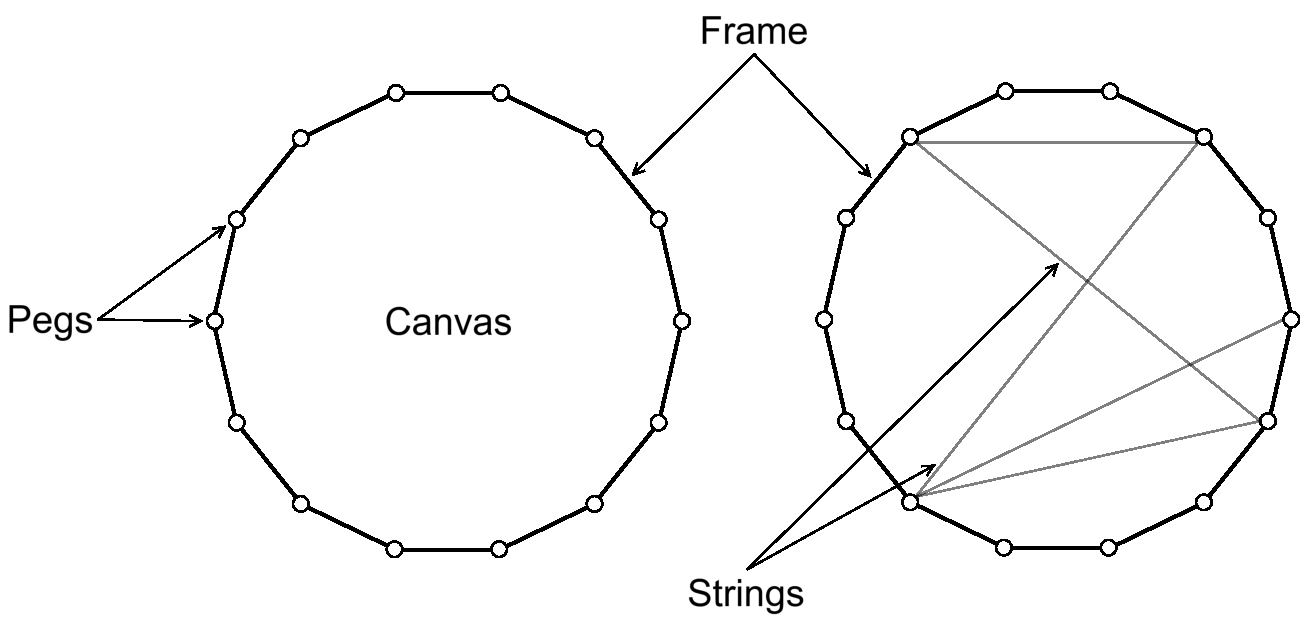
\includegraphics[width=\linewidth]{images/stringart_components.pdf}
                \caption{Componente ale artei cu sfoară.}
            \end{figure}
        \end{column}
    \end{columns}
\end{frame}
%------------------------------------------------

%------------------------------------------------
\section{Definirea problemei}
\begin{frame}{Definirea problemei}
    \begin{figure}
        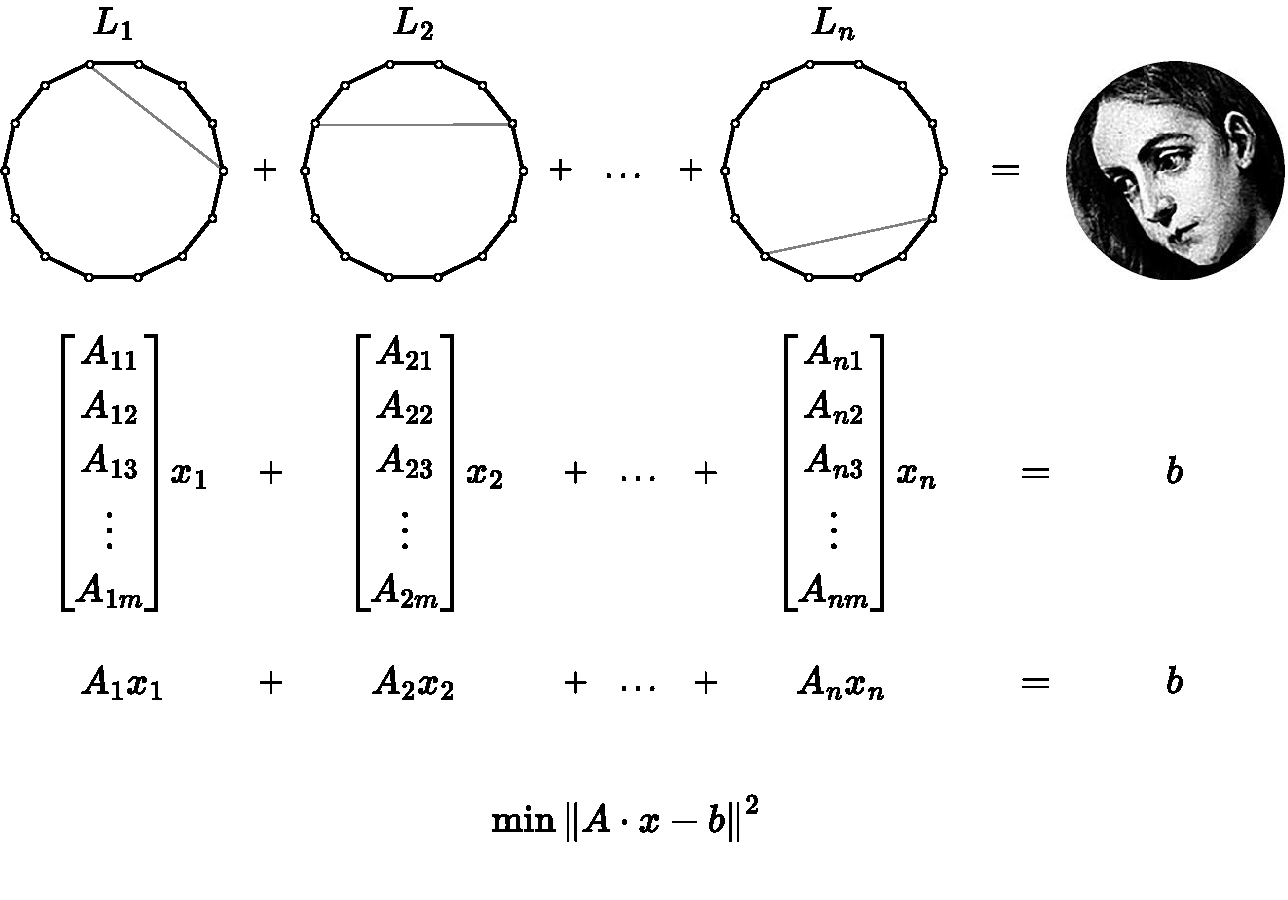
\includegraphics[width=0.75\linewidth]{images/problem_definition.pdf}
    \end{figure}
\end{frame}
%------------------------------------------------

%------------------------------------------------
\section{Metodologie}
\begin{frame}{Transformata Radon}
    \begin{figure}[H]
    \centering
        \begin{minipage}{0.5\linewidth}
            \centering
            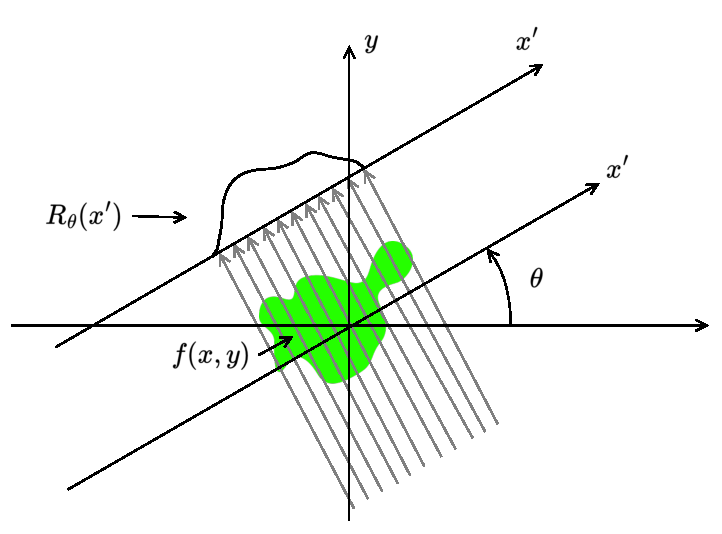
\includegraphics[width=\linewidth]{images/radon.pdf}
        \end{minipage}
    \hspace{0.02\linewidth}
        \begin{minipage}{0.2\linewidth}
            \centering
            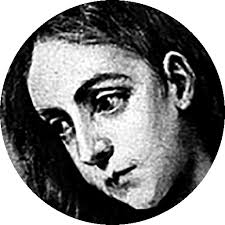
\includegraphics[width=\linewidth]{images/mary.png}
        \end{minipage}
    \hspace{0.02\linewidth}
        \begin{minipage}{0.2\linewidth}
            \centering
            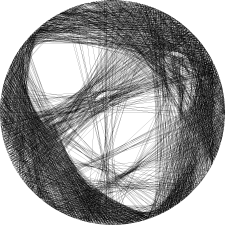
\includegraphics[width=\linewidth]{images/mary_radon.png}
        \end{minipage}
\end{figure}
\end{frame}

\begin{frame}{Analiză Comparativă Metode cu Coeficienți Binari}
    \begin{figure}
        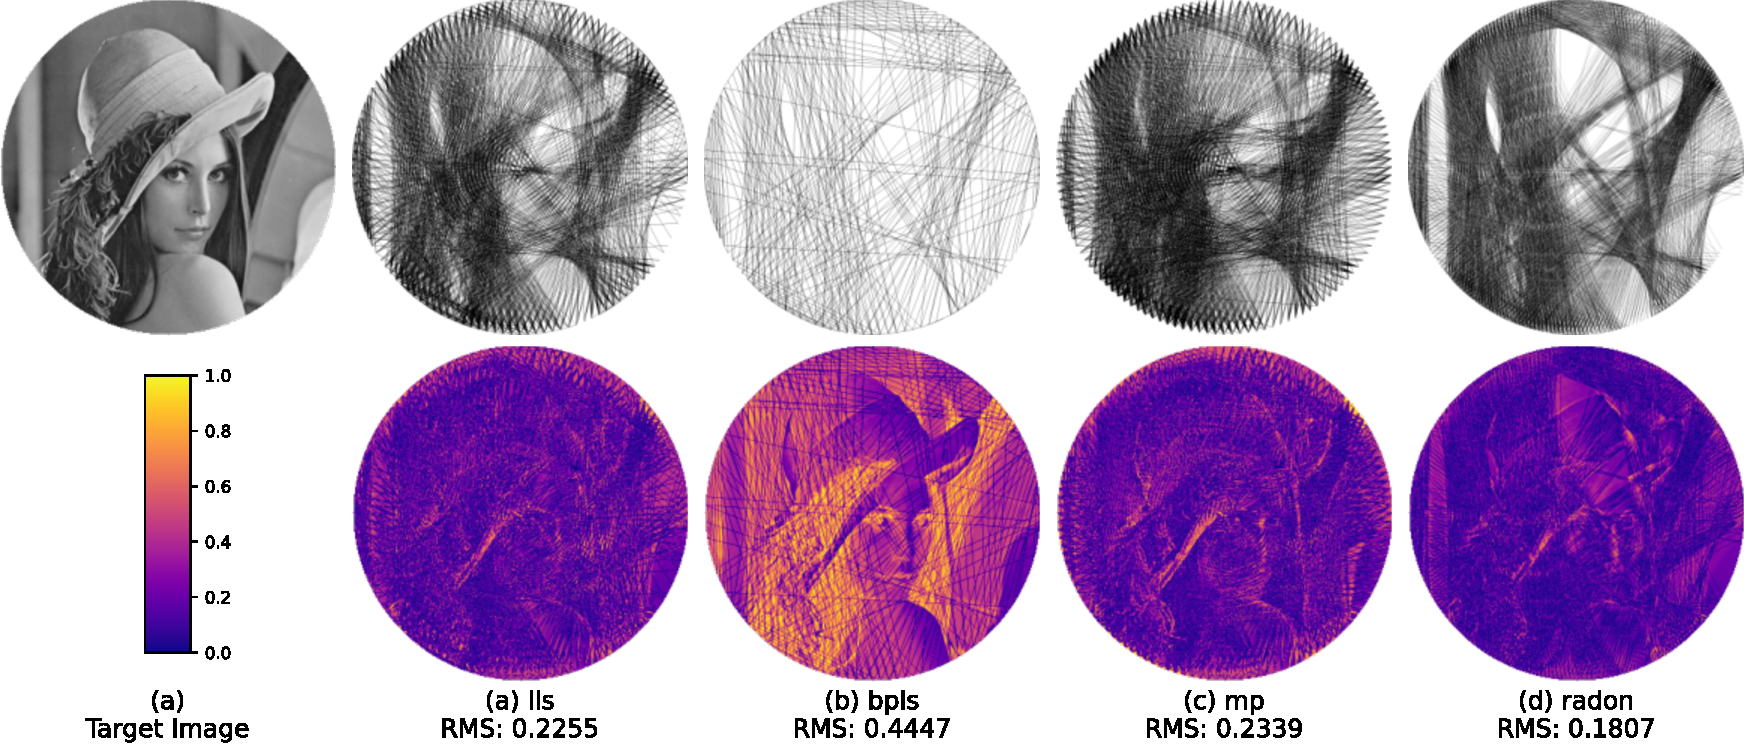
\includegraphics[width=0.9\linewidth]{images/diff_images_binary.pdf}
    \end{figure}
\end{frame}

\begin{frame}{Analiză Comparativă Metode cu Coeficienți Reali}
    \begin{figure}
        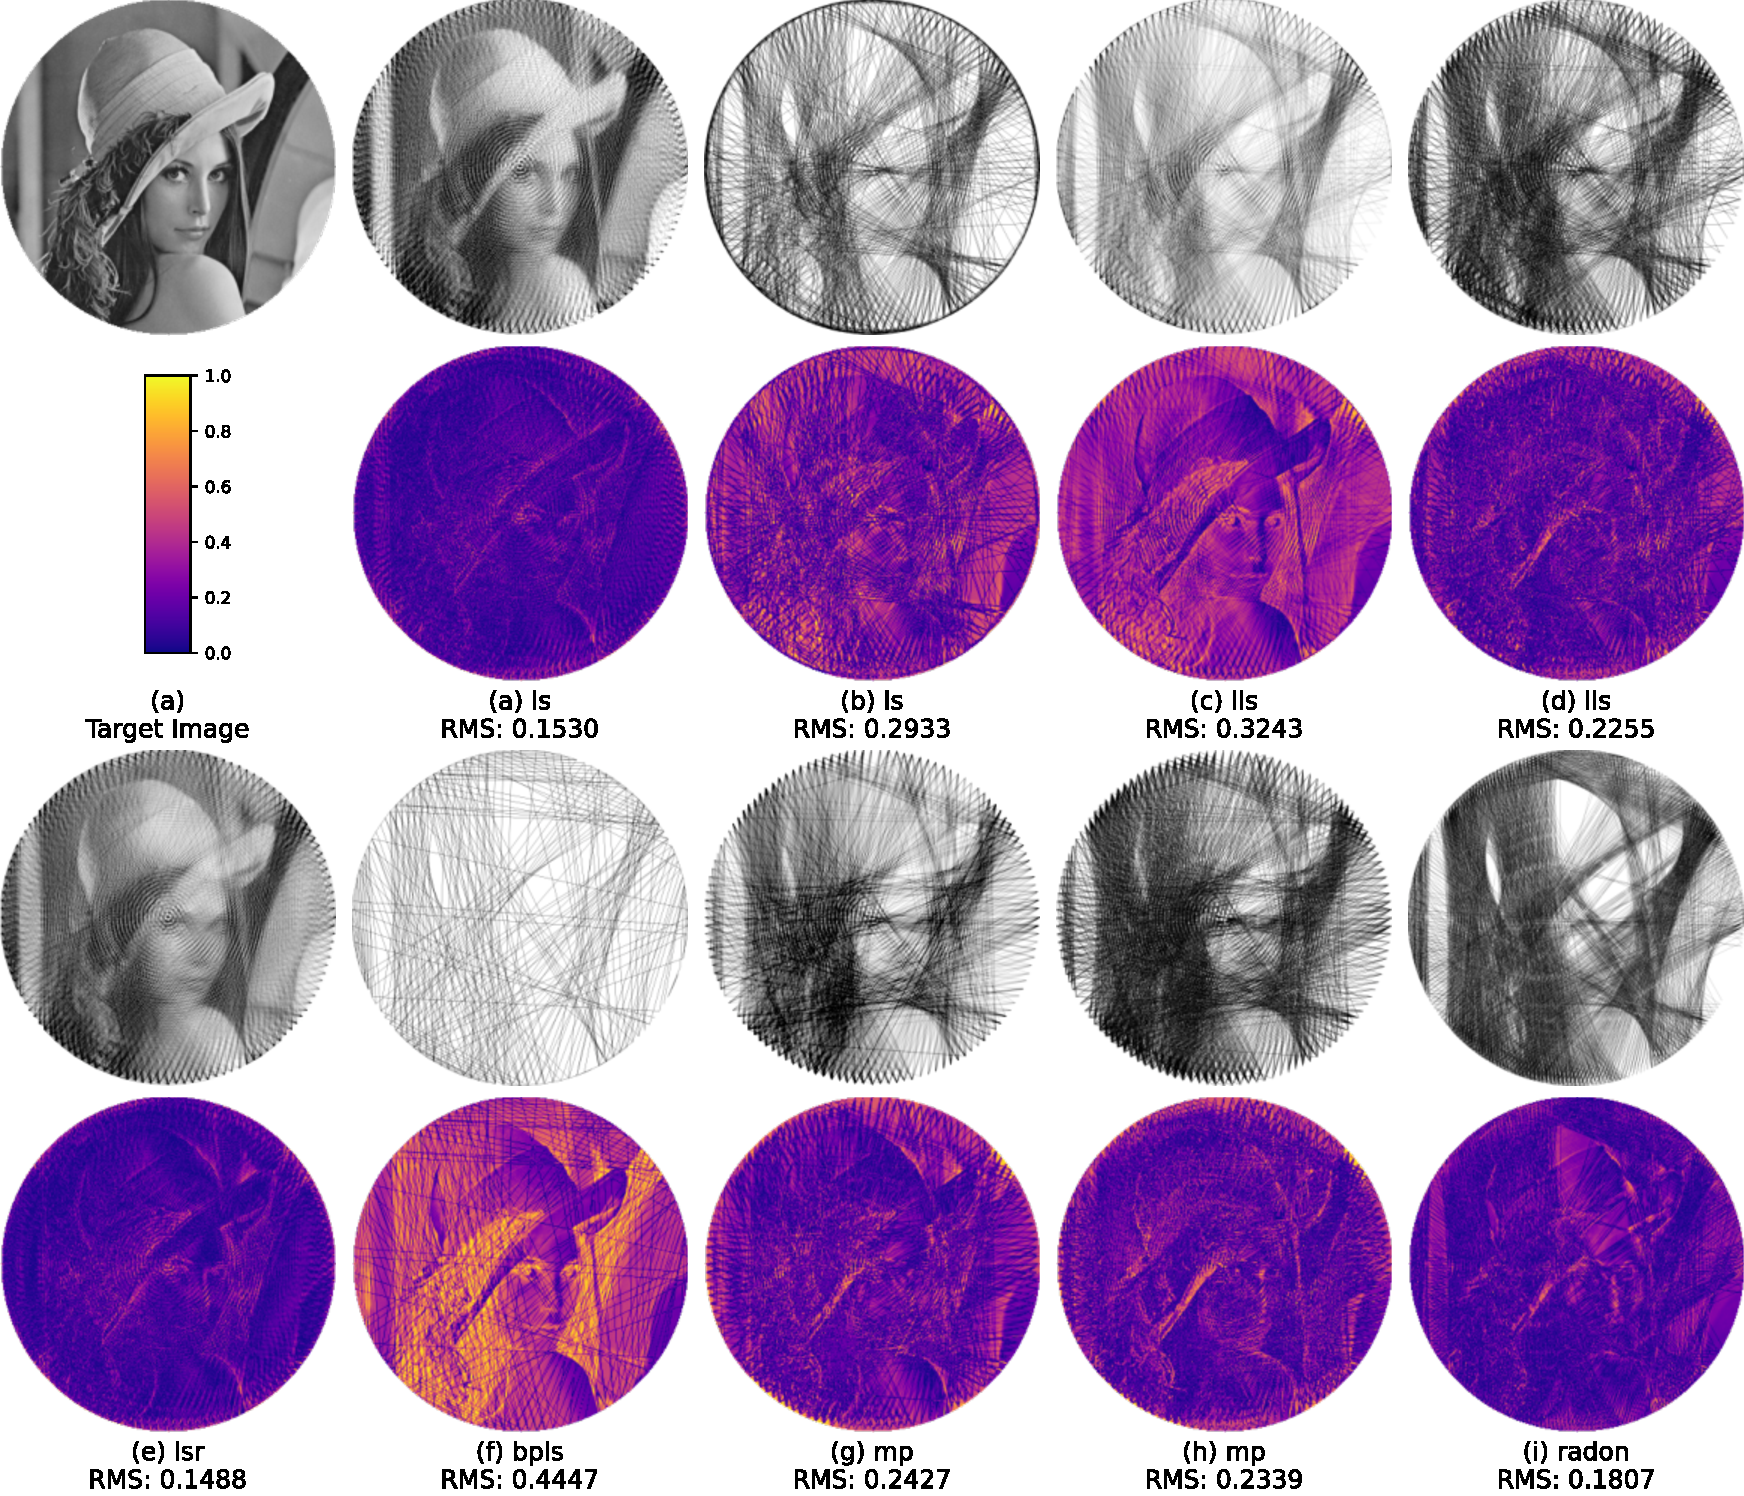
\includegraphics[width=0.9\linewidth]{images/diff_images.pdf}
    \end{figure}
\end{frame}

\begin{frame}{Istoric Reziduu}
    \begin{figure}
        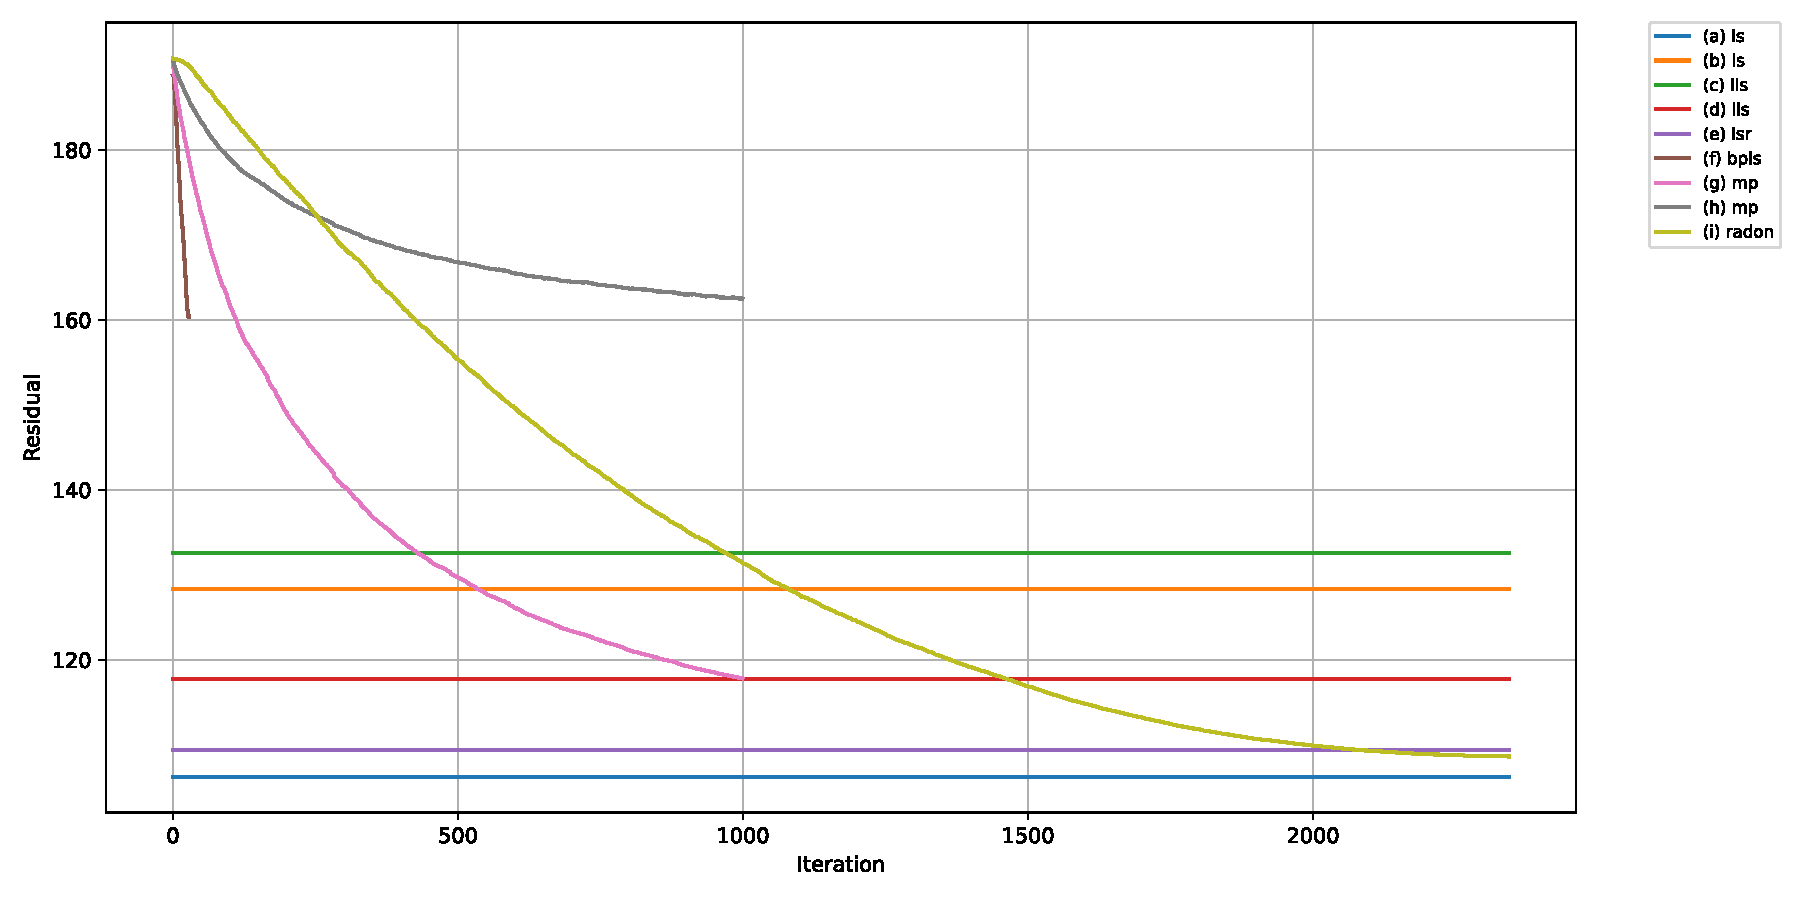
\includegraphics[width=0.9\linewidth]{images/residual_history.pdf}
    \end{figure}
\end{frame}

\begin{frame}{Rezultate Cantitative Radon}
    \begin{figure}
        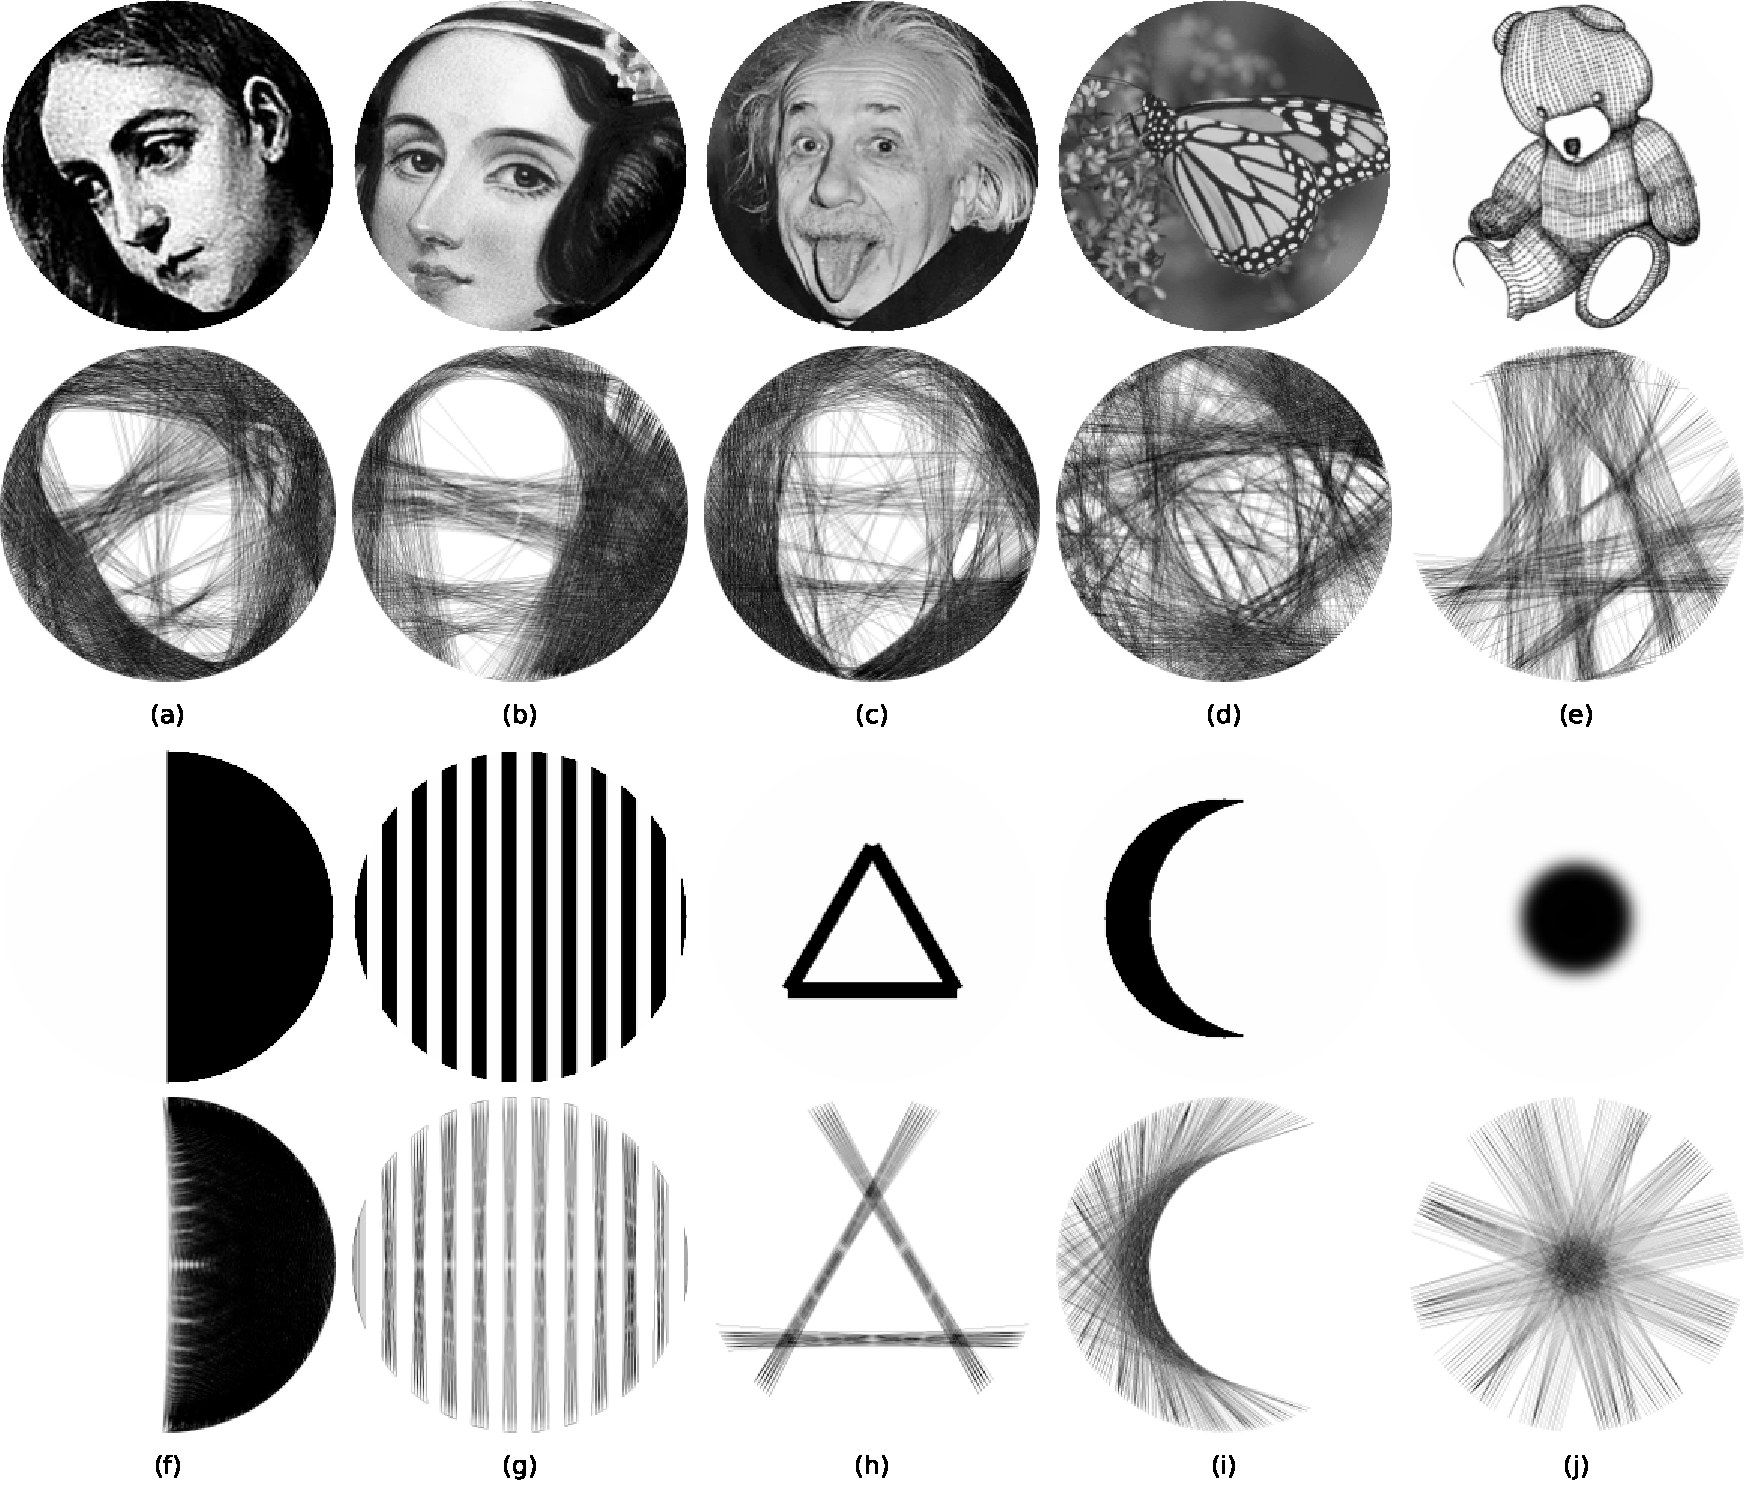
\includegraphics[width=0.6\linewidth]{images/radon_quantitative_test.pdf}
    \end{figure}
\end{frame}
%------------------------------------------------

%------------------------------------------------
\section{Sumar și Perspective}
\begin{frame}{Concluzie}
    \textbf{Cea mai bună metodă: Radon}
    \begin{itemize}
        \item Produce un rezultat binar, cu un contrast bun și separare clară între fundal și subiect.
        \item De \textbf{6.7× mai rapidă} decât BPLS, dar \textbf{12.6× mai lentă} decât LLS binar.
        \item De \textbf{8× mai eficientă} în memorie decât BPLS, dar \textbf{1.62× mai consumatoare} decât LLS binar.
        \item RMS competitiv: \textbf{0.1807} —  LLS binar (0.2255), BPLS (0.4447), MP binar (0.2339).
    \end{itemize}

    \vspace{0.5cm}

    \textbf{Perspective viitoare}
    \begin{itemize}
        \item Explorarea metodei de transfer de stil bazată pe deep learning a fost deja începută.
        \item Direcție propusă: dezvoltarea unui model care să prezică direct liniile folosite, nu doar să aplice un stil.
    \end{itemize}
\end{frame}
%------------------------------------------------

\end{document}